\question{Определенный интеграл. Определение, свойства линейности и аддитивности.}

\underline{Постановка задачи}: требуется найти площадь криволинейной фигуры.
Разобьем фигуру на квадраты и найдем площадь каждого из них. После это сложим
полученные площади.

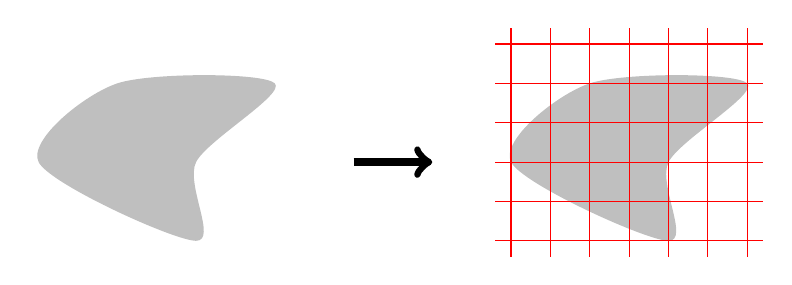
\begin{tikzpicture}
  \def\Shift{6}
  \fill[lightgray] plot [smooth cycle] coordinates {
    (0, 0) (1, 1) (3, 1) (2, 0) (2, -1)
  };
  \draw[->, line width = 1mm] (\Shift - 2, 0) -- (\Shift - 1, 0);
  \fill[lightgray] plot [smooth cycle] coordinates {
    (\Shift, 0) (\Shift + 1, 1) (\Shift + 3, 1) (\Shift + 2, 0) (\Shift + 2, -1)
  };
  \draw[step = 0.5, red, thin] (\Shift - 0.2, -1.2) grid (\Shift + 3.2, 1.7);
\end{tikzpicture}


Упростим задачу: пусть нужно посчитать площадь криволинейной трапеции.

\begin{minipage}{\linewidth}
  \begin{multicols*}{2}
    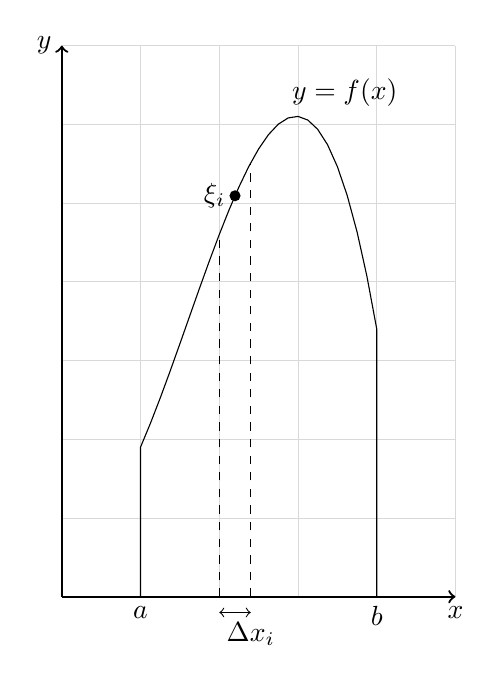
\begin{tikzpicture}
  \draw[very thin, gray!30, step = 1cm] (0, 0) grid (5, 7);
  \draw[domain = 1 : 4, variable = \x]
    (1, 0)
    -- plot ({\x}, {-0.5 * \x * \x * \x + 2.4 * \x * \x - \x + 1})
    -- (4, 0)
    -- cycle;

  \draw[<->] (2, -0.2) -- (2.4, -0.2) node [below] {\(\Delta x_{i}\)};
  \draw[dashed] (2, 0) -- (2, 4.6);
  \draw[dashed] (2.4, 0) -- (2.4, 5.512);
  \draw node[above, left] at (2.2, 5.092) {\(\xi_{i}\)};
  \fill[black] (2.2, 5.092) circle (2pt);

  \draw[thick] [->] (0, 0) -- (5, 0) node[right, below] {\(x\)};
  \draw[thick] [->] (0, 0) -- (0, 7) node[above, left] {\(y\)};
  \draw node[right] at (2.8, 6.4) {\(y = f(x)\)};
  \draw node[below] at (1, 0) {\(a\)};
  \draw node[below] at (4, 0) {\(b\)};
\end{tikzpicture}

    \columnbreak

    \begin{enumerate}
      \item Разбиение области \([a;b]\):
      \(a = x_{0} < x_{1} < \dotsc < x_{n} = b\).
      Отрезок \([x_{i - 1}, x_{i}]\) назовем частичным, если длину обозначим 
      \(\Delta x_{i} = x_{i} - x_{i - 1}\).
      Разбиение (дробление) обозначим \(T = \{ x_{i} \}_{i = 0}^{n}\). Введем
      понятие \textit{ранга} дробления \(\tau\): \(\tau = \max \Delta x_{i}\).

      \item Выберем среднюю точку \(\xi_{i} \in [x_{i - 1}, x_{i}]\). Тогда
      \(f(\xi_{i})\) это высота элементарного прямоугольника. Значит площадь
      элементарного прямоугольника будет равна
      \(S_{e} = f(\xi_{i}) \Delta x_{i}\).

      \item Просуммируем площади всех элементарных прямоугольников:
      \(\sum_{i = 1}^{n} f(\xi_{i}) \Delta x_{i}\). Данная сумма называется
      интегральной суммой Римана.

      \item Возьмем предел при \(n \to \infty\) и \(\tau \to 0\):
      
      \begin{align*}\label{eq:lim-int-sum}\tag{1}
        \lim_{\substack{n \to \infty \\ \tau \to 0}}
          \sum_{i = 1}^{n} f(\xi_{i}) \Delta x_{i}
      \end{align*}
    \end{enumerate}
  \end{multicols*}
\end{minipage}

\begin{definition}
  Если полученный предел интегральных сумм \eqref{eq:lim-int-sum} существует,
  конечен, \textbf{не зависит от дробления и выбора средней точки},то он
  называется определенным интегралом.

  \begin{align*}
    \int_{a}^{b} f(x) \dd x = \lim_{\substack{n \to \infty \\ \tau \to 0}}
      \sum_{i = 1}^{n} f(\xi_{i}) \Delta x_{i}
  \end{align*}

  \(a, b\) называются пределами интегрирования, \(f(x)\)~--- подынтегральной
  функцией, а \(\dd x\)~--- дифференциалом переменной (или элементом длины).
\end{definition}

\begin{remark}\label{def-int-ad}
  В определении выше \(a < b\). Доопределим для случаев \(a = b\) и \(a > b\):

  \begin{align*}
    \int_{a}^{a} f(x) \dd x = 0 \qquad
    \int_{a}^{b} f(x) \dd x = -\int_{b}^{a} f(x) \dd x
  \end{align*}
\end{remark}

\begin{remark}
  Интеграл Римана определен для кусочно-непрерывных (т.е. имеющих конечное
  число разрывов) функций.
\end{remark}

Т.к. интеграл является пределом сумм, то его свойства вытекают из свойств
пределов:
\begin{enumerate}
  \item Линейность
  
  \begin{align*}
    \int_{a}^{b} (\lambda f(x) + \mu g(x)) \dd x =
    \lambda \int_{a}^{b} f(x) \dd x + \mu \int_{a}^{b} g(x) \dd x
  \end{align*}

  \item Аддитивность
  
  \begin{align*}
    \int_{a}^{b} f(x) \dd x =
    \int_{a}^{c} f(x) \dd x + \int_{c}^{b} f(x) \dd x
  \end{align*}
\end{enumerate}

\begin{remark}
  Свойство аддитивности выполняется даже в случае, если \(c \notin [a;b]\). Это
  легко проверить пользуясь свойством \ref{def-int-ad}.
\end{remark}